\section{Eksperymenty}
Teraz chciałbym pokazać jak działa moja aplikacja. W tym celu spróbuję trochę poeksperymentować z danymi i pokazać to, co do tej pory udało się osiągnąć.

\subsection{Reguła z jednym warunkiem i jedną akcją}
Wyobraźmy sobie sytuację że robimy system rejestrujący badania medyczne wykonane na rzecz pacjenta. Chcielibyśmy się dowiedzieć, czy rejestrowane badanie jest badaniem refundowanym (nasza wyobrażona refundacja dotyczy tylko badań zarejestrowanych w roku 2019). O czasie rejestracji badania mówi zmienna ,,data\_rejestracji\_badania''. W przypadku gdy badanie nie jest refundowane system ma wyświetlić komunikat informacyjny. 

Na początek definicja reguły, niech brzmi ona następująco:
\\ \\
\fbox{\begin{minipage}{40em}
\textit{Jeżeli data\_rejestracji\_badania jest mniejsza niż '01-01-2019' wtedy wyświetl komunikat "Badanie sprzed okresu refundacji".}
\end{minipage}}
\\ \\
Wprowadzam ją do systemu, i wygląda to tak:
\begin{figure}[H]
	\centering
	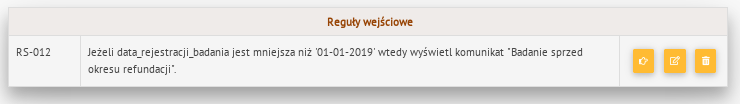
\includegraphics[scale=0.8]{img/app-eksperymenty/p1-1.png}
\end{figure}

\newpage
Teraz spójrzmy czego udało się o niej dowiedzieć:
\begin{figure}[H]
	\centering
	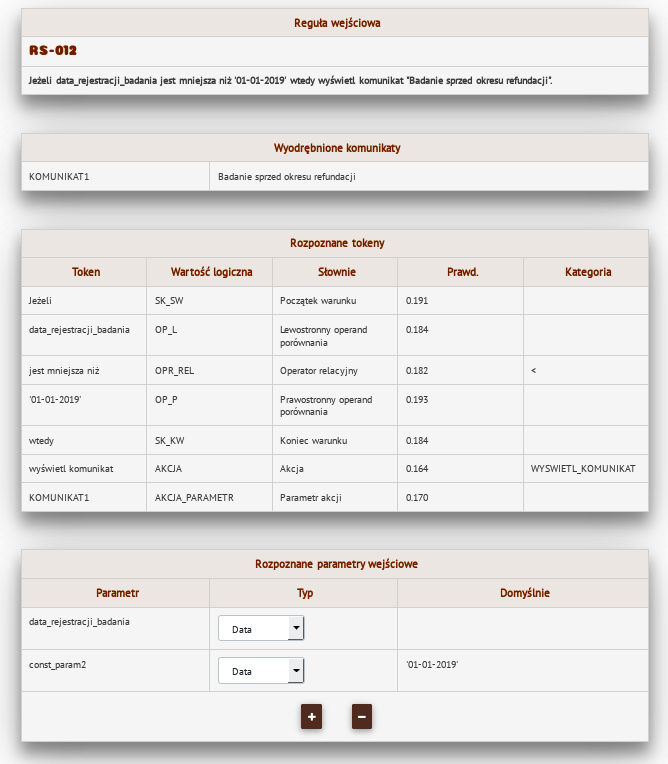
\includegraphics[scale=0.9]{img/app-eksperymenty/p1-2.png}
\end{figure}

\begin{itemize}
	\item \textbf{Reguła wejściowa} - system jeszcze raz przypomina treść wprowadzonej reguły i prezentuje nadany jej kod, w naszym przypadku RS-012.
	\item \textbf{Wyodrębnione komunikaty} - tu zaprezentowane zostały komunikaty, które udało się wyszukać w regule. Każdy odnaleziony komunikat zostaje wycięty z reguły przed poddaniem jej analizie i zastąpiony swoim reprezentującym go identyfikatorem - w naszym przypadku odnaleziony został jeden komunikat i zastąpiony przez słowo \textit{,,KOMUNIKAT1''}.
	\item \textbf{Rozpoznane tokeny} - najistotniejsza część wyników analizy. Widzimy, że z tą regułą algorytm poradził sobie bezbłędnie. Tokeny zostały prawidłowo skojarzone z ich znaczeniem logicznym. \\
	Na chwilę uwagi zasługuje tylko kolumna ,,Kategoria'' . Dotyczy ona tych tokenów, które mogą być określone na wiele sposobów. Musimy przyporządkować im jedną, uniwersalną kategorię. Jako przykład niech posłuży operator mniejszości - może on zostać opisany jako (,,jest mniejszy niż'',,,jest mniejszy od'',,,jest mniejsza od'',\dots). Z punktu widzenia aplikacji, wszystkie te wartości reprezentują jedną kategorią, ja nazwałem ją po prostu ,,<'' .
	\item {Rozpoznane parametry wejściowe} - w tym miejscu pokazywane są wartości, które uznane zostały za parametry wejściowe reguły. Trafiają tu tokeny, które biorą udział w porównaniach, lub są przekazywane jako parametry wejściowe do innych reguł (tę sytuację pokażę trochę później). W tym przypadku widzimy, że aplikacji udało się prawidłowo dopasować typy danych i określić wartość domyślną jednego z parametrów. Gdyby to się nie udało, czynność tę musi wykonać człowiek. Musi się to stać przed wygenerowaniem kodu.
\end{itemize}


I na koniec spójrzmy na wygenerowany kod metody walidującej regułę RS-012.
\begin{figure}[H]
	\centering
	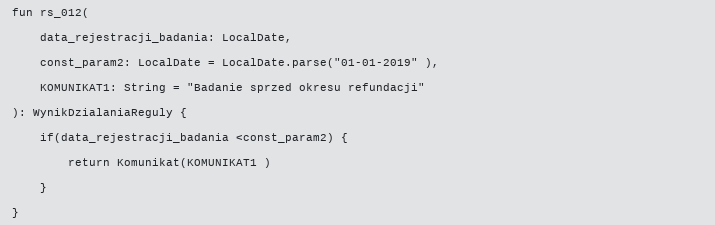
\includegraphics[scale=0.8]{img/app-eksperymenty/p1-3.png}
\end{figure}

Wszystko wygląda ok, więc spróbujmy trochę skomplikować regułę. 

\subsection{Reguła z podwójnym warunkiem}
Załóżmy że refundacji podlegają tylko te badania, które zostały wykonane w pierwszym kwartale 2019 roku. Chcielibyśmy zmienić treść reguły w taki sposób, by po stwierdzeniu tego typu sytuacji informowała użytkownika że jego badanie może zostać zrefundowane.
\\ \\
\fbox{\begin{minipage}{40em}
		\textit{Jeżeli data\_rejestracji\_badania jest większa niż '01-01-2019' i data\_rejestracji\_badania jest mniejsza od '01-04-2019' wtedy wyświetl komunikat "Badanie podlega refundacji".}
\end{minipage}}
\\ \\
Modyfikujemy regułę:
\begin{figure}[H]
	\centering
	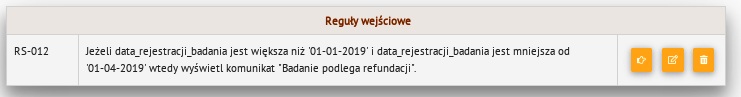
\includegraphics[scale=0.8]{img/app-eksperymenty/p2-1.png}
\end{figure}
I oglądamy wyniki:
\begin{figure}[H]
	\centering
	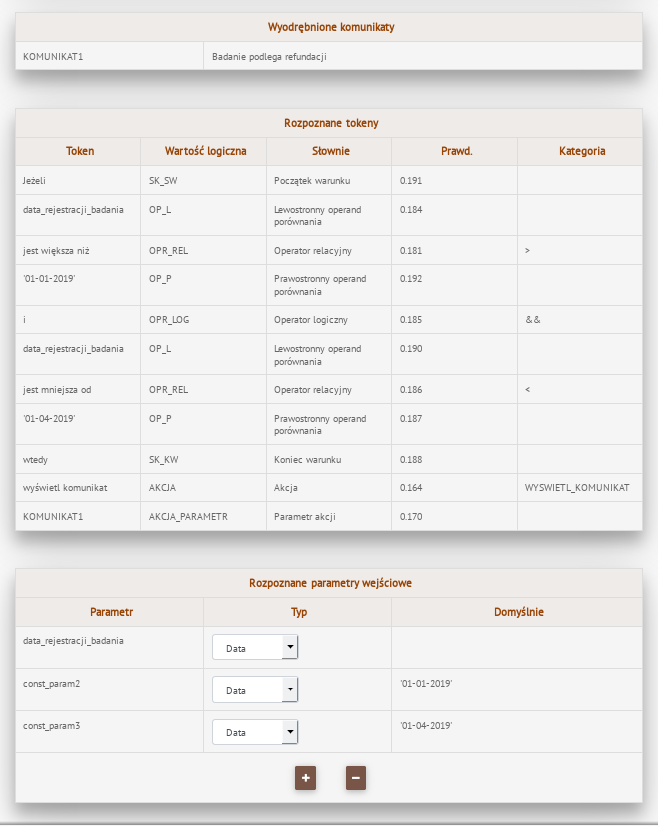
\includegraphics[scale=0.8]{img/app-eksperymenty/p2-2.png}
\end{figure}
Istotne zmiany doszły w tabeli rozpoznanych tokenów. Doszedł operator logiczny, oraz druga część warunku. Udało się również prawidłowo przyporządkować operatory do określających je kategorii. Dodatkowo pojawił się nowy parametr wejściowy, który definiuje drugą z porównywanych wartości. 

Wygenerowany kod również wygląda na poprawny:
\begin{figure}[H]
	\centering
	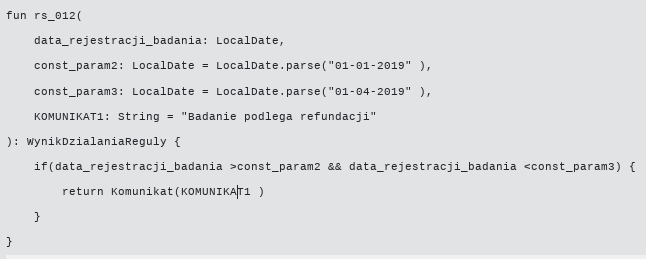
\includegraphics[scale=0.8]{img/app-eksperymenty/p2-3.png}
\end{figure}

\subsection{Reguła z akcją ,,w przeciwnym wypadku''}
Załóżmy, że chcielibyśmy by  w przypadku spełnienia warunku reguła wyświetlała stosowny komunikat informacyjny, a w przypadku gdy warunek nie zostanie spełniony zwracała błąd walidacji . \\
Będzie ona miała następującą postać:
\\ \\
\fbox{\begin{minipage}{40em}
		\textit{Jeżeli data\_rejestracji\_badania jest większa niż '01-01-2019' i data\_rejestracji\_badania jest mniejsza od '01-04-2019' wtedy wyświetl komunikat "Badanie podlega refundacji", w przeciwnym wypadku zgłoś błąd "Badanie nie może zostać zarejestrowane" .}
\end{minipage}}
\\ \\
Tak jak poprzednio, dokonujemy zmian w treści reguły:
\begin{figure}[H]
	\centering
	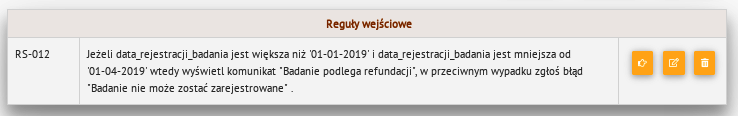
\includegraphics[scale=0.8]{img/app-eksperymenty/p3-1.png}
\end{figure}

W tabeli rozpoznanych tokenów znowu pojawiły się nowe rekordy. Tym razem doszła sekcja związana z akcją ,,NIE''. Wygląda na to, że algorytm poradził sobie również z tą regułą i prawidłowo określił znaczenie poszczególnych słów.

\begin{figure}[H]
	\centering
	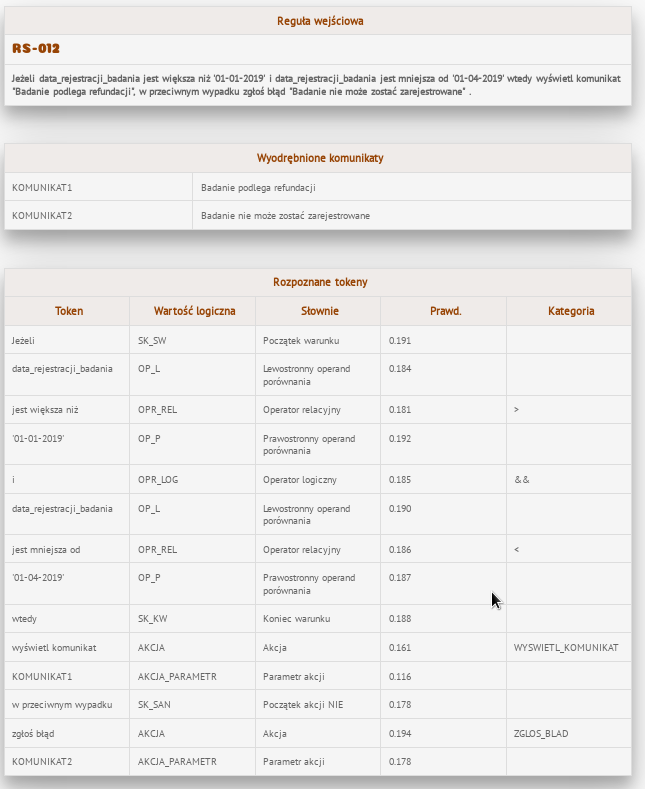
\includegraphics[scale=0.8]{img/app-eksperymenty/p3-2.png}
\end{figure}
Zmiany zaszły również w wygenerowanym kodzie. Nasza instrukcja warunkowa otrzymała część ,,ELSE'', a metoda zwraca nowy typ obiektu.
\begin{figure}[H]
	\centering
	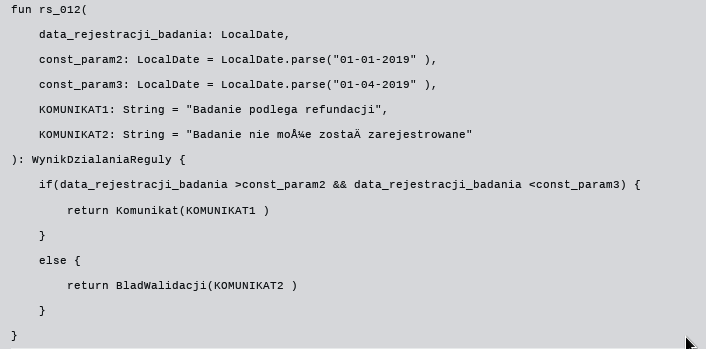
\includegraphics[scale=0.8]{img/app-eksperymenty/p3-3.png}
\end{figure}

\subsection{Reguła z wywołaniem innej reguły}
W tym scenariuszu założymy, że sprawdzanie warunków dat refundacji badania ma odbyć się tylko wtedy, gdy spełniony zostanie warunek odpowiedniego wieku pacjenta. Żeby go zrealizować definiujemy nową regułę o następującej treści:
\\ \\
\fbox{\begin{minipage}{40em}
		\textit{dy wiek\_pacjenta jest większy od 18 wtedy zgłoś wyjątek "Przekroczony wiek refundacji", w przeciwnym wypadku sprawdzaj regułę RS-012 .}
\end{minipage}}
\\ \\

\begin{figure}[H]
	\centering
	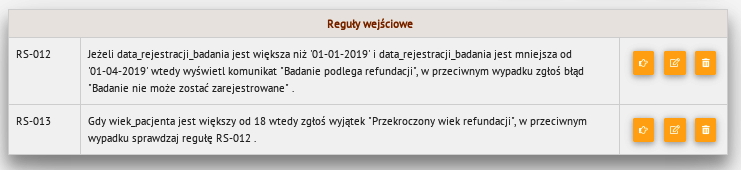
\includegraphics[scale=0.8]{img/app-eksperymenty/p4-1.png}
\end{figure}
Po przejściu do sekcji analizy wyników od razu można zauważyć że pojawiły się nam błędy walidacji  i niemożliwe jest poprawne wygenerowanie kodu.
\begin{figure}[H]
	\centering
	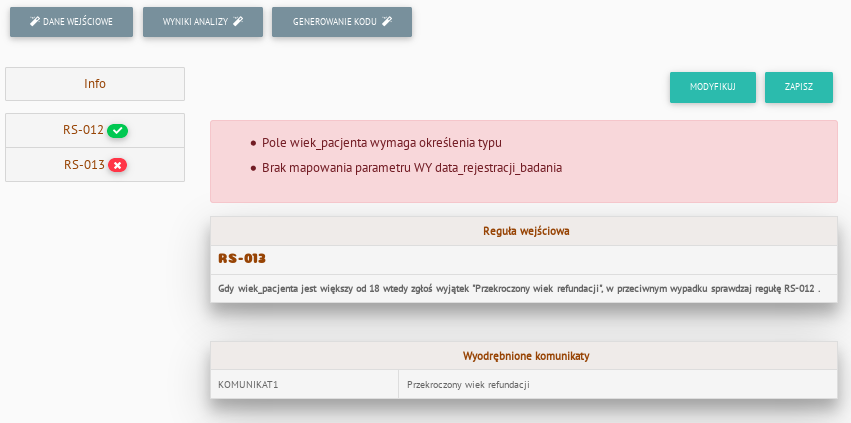
\includegraphics[scale=0.7]{img/app-eksperymenty/p4-1_5.png}
\end{figure}
W sekcji tokenów wszystko wygląda w porządku. Warunki, słowa kluczowe oraz akcje rozpoznane zostały poprawnie.  

\begin{figure}[H]
	\centering
	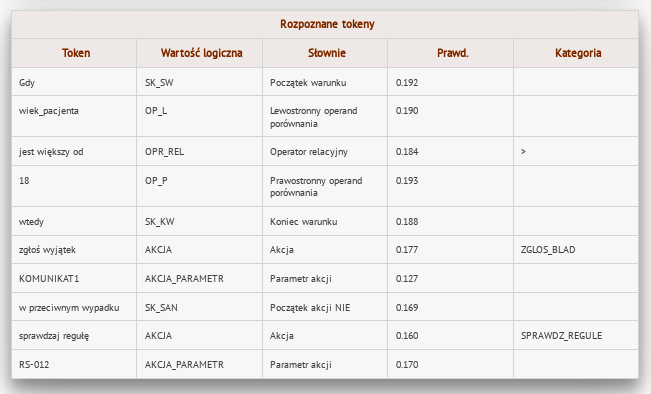
\includegraphics[scale=0.8]{img/app-eksperymenty/p4-2.png}
\end{figure}

Pierwszy problem napotykamy w sekcji ,,Parametrów wejściowych''. Aplikacja prawidłowo rozpoznała zmienną ,,wiek\_pacjenta'' jako parametr, ale z treści reguły nie da się wywnioskować jakiego on jest typu. Wymagana jest pomoc użytkownika. Z listy rozwijanej należy wybrać opcję ,,Liczba''. To załatwia temat pierszego z błędów.
\begin{figure}[H]
	\centering
	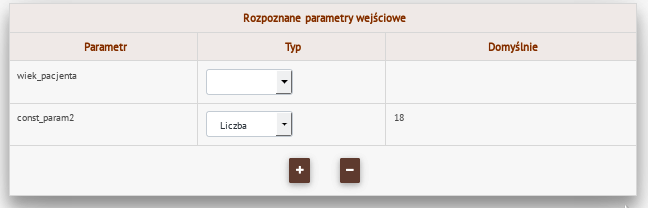
\includegraphics[scale=0.8]{img/app-eksperymenty/p4-3.png}
\end{figure}

Kolejny problem dotyczy samego wywołania reguły ,,RS-012''. Reguła ta na wejściu oczekuje podania daty. W tabeli wywołania użytkownik musi zmapować który parametr wejściowy reguły ,,RS-013'' ma zostać przekazany na wejście reguły ,,RS-012''. I tu pojawia się nowy problem, ponieważ reguła ,,RS-013'' tej daty nie przyjmuje. 

\begin{figure}[H]
	\centering
	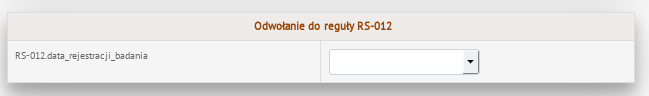
\includegraphics[scale=0.8]{img/app-eksperymenty/p4-4.png}
\end{figure}

Konieczne jest cofnięcie się do tabeli parametrów i użycie opcji dodania nowego parametru - niech nazywa się on ,,data\_badania'' i będzie miał typ ,,Data''. Po tym kroku możliwe staje się wykonanie odpowiedniego przemapowania i po zapisaniu błędy walidacji znikają.
\begin{figure}[H]
	\centering
	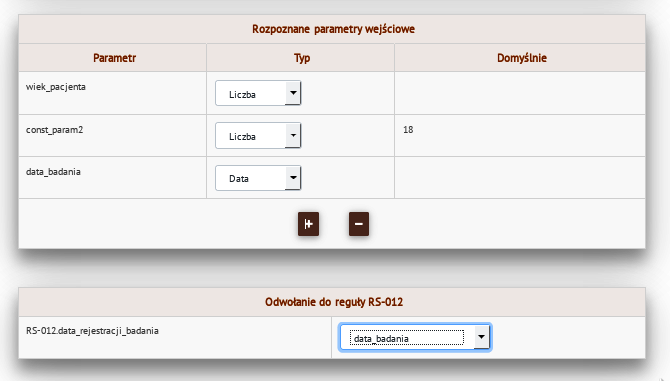
\includegraphics[scale=0.8]{img/app-eksperymenty/p4-5.png}
\end{figure}

Poniżej kod, który teraz już bez przeszkód udało się wygenerować:

\begin{figure}[H]
	\centering
	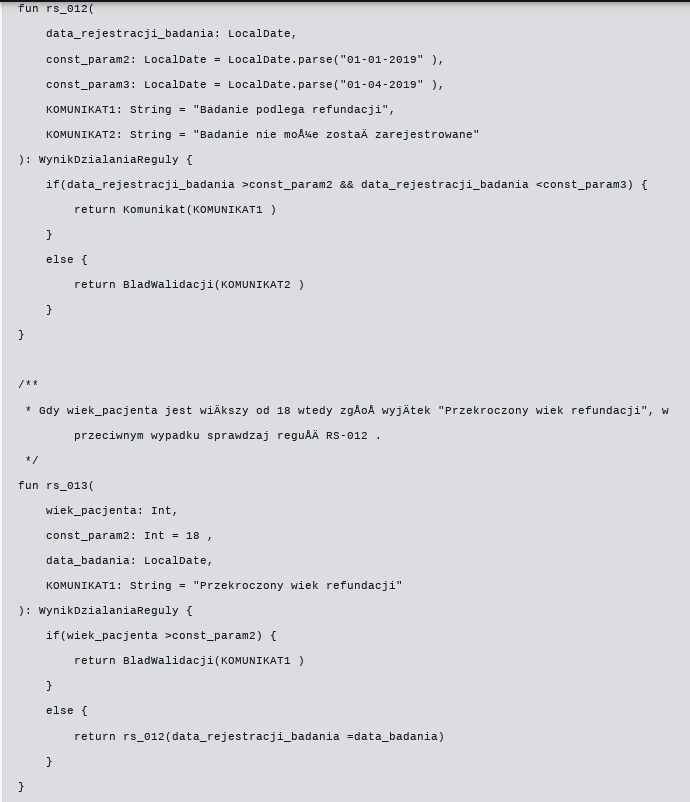
\includegraphics[scale=0.8]{img/app-eksperymenty/p4-6.png}
\end{figure}